%!TEX root = ../document.tex

\section[Design Thinking (Author: Felix Leupold)]{Design Thinking}
\label{sec:DESIGN_THINKING}

\emph{Design thinking} refers to the method of finding an innovative solution to an abstract or ill-defined problem. It attempts to structure the ideation process and provides guidelines, methodologies and frameworks that help in problem forming, -solving and -design. Design thinking is a human-centered approach with multidisciplinary collaboration and iterative improvements to produce innovative products, systems and services \cite{design_thinking_book}. There are various interpretations and definitions of design thinking. We refer to design thinking as defined by the Hasso Plattner Institue of Design at Stanford and Potsdam. In this definition the design thinking process contains six different phases, which are pictured in Figure \ref{fig:design_thinking_process}. The process is not linear, which is indicated by the connections amongst different non-succeeding phases. Every instance of a design thinking project is different. It is possible to jump back and forth between the different phases as you encounter new inflection points. 

%nochmal �berdenken
In the following, we briefly explain the aim of each phase as they also reflect the pathway in the course of our project and the structure of this report.

\begin{figure}
    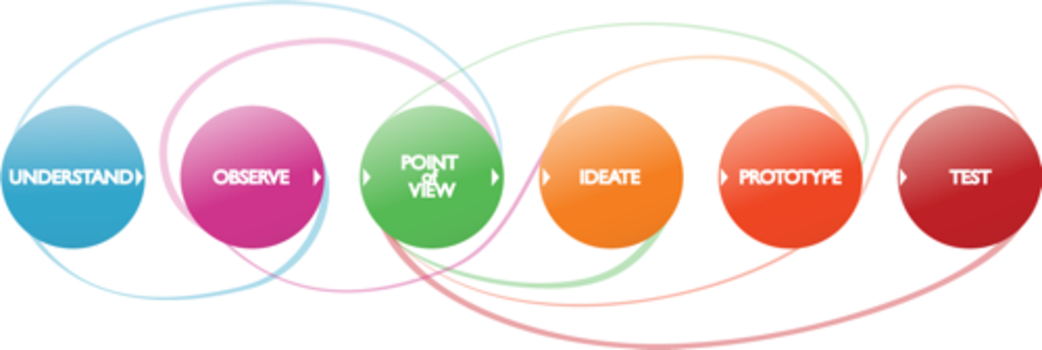
\includegraphics[width=\linewidth]{images/design_thinking_process}
    \caption{Design Thinking process according to \emph{Hasso Plattner Institue of Design} at Stanford and Potsdam.}
    % #selfrespect
    \label{fig:design_thinking_process}
\end{figure}

\paragraph{Understand}
In the first phase of the process, the team becomes familiar with the problem domain by talking to experts and conducting research. The goal is to develop background knowledge through these experiences. It is the foundation for all further steps. Throughout the process this stage might be visited again as new areas of problems, ideas or solutions emerge.

\paragraph{Observe}
What people say does not always correspond to their actual feelings, thoughts or actions. Therefore, it is necessary to watch how people behave and interact. These observations can be used to talk to users, ask questions and reflect on their behaviors. They lay the foundation for insights which are needed to define a point of view later in the process. Another point of this phase is to develop a kind of empathy for the user.

\paragraph{Point Of View}
The point of view consists of three parts: A persona, which is a concrete specification of the target user the team is designing for. Second, a need that this persona has and that the team is trying to satisfy with its solution. Lastly, an insight that has been generated from the observation made in the second phase. A commonly used method of defining a point of view is the "How might we..." question, which is a statement in a form "How might we help our persona to satisfy his or her need".
While the preceding phases tried to capture a wide range of users and problems, in this stage the team settles on a single point from which it can converge again in the next phase.

\paragraph{Ideate}
While the first three phases focus on defining and understanding the problem, the ideation phase opens up the solution space for the problem. The team is challenged to brainstorm as many solutions as possible by going for quantity, deferring judgment and building on the ideas of others.

\paragraph{Prototype}
Prototyping is a crucial part of the design thinking process. It allows to make the ideas visible and tangible. Quick and cheap prototypes, e.g. sketches on paper, are well suited for conveying the idea and getting feedback. People tend to hesitate to criticize or suggest changes for overly polished prototypes. A key concept is to fail early and often.

\paragraph{Test}
In the test phase the team collects feedback on their ideas which they made experienceable through their prototype. The goal of this phase is to learn which parts of the design work and which don't.
Testing ensures that the product is desirable for the end user and stresses the user focus of design thinking.
Latest from here on the team continues with one of the earlier phases.

\paragraph{}
Each potential solution has to satisfy three requirements as depicted in Figure \ref{fig:desire_viable_feasible}. Desirability ensures, it addresses an actual need of the user. Feasibility means that the solution should be technically possible to implement. Lastly, it has to be viable for the business partner providing the solution.
Innovative solutions lie in the intersection of the three sets. Design thinking helps to find solutions that lie in this intersection.

\begin{figure}
\begin{centering}
    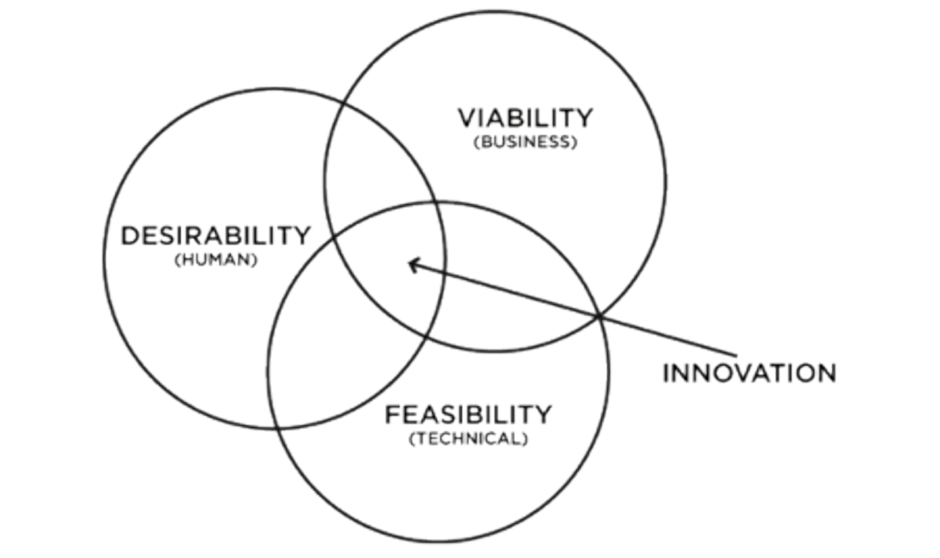
\includegraphics[width=0.5\linewidth]{images/desire_viable_feasible}
    \caption{Solution can be categorized into different sets. An innovative solution has to be viable, desirable and feasible.}
    % #selfrespect
    \label{fig:desire_viable_feasible}
\end{centering}
\end{figure}